% Options for packages loaded elsewhere
\PassOptionsToPackage{unicode}{hyperref}
\PassOptionsToPackage{hyphens}{url}
%
\documentclass[
]{book}
\usepackage{lmodern}
\usepackage{amssymb,amsmath}
\usepackage{ifxetex,ifluatex}
\ifnum 0\ifxetex 1\fi\ifluatex 1\fi=0 % if pdftex
  \usepackage[T1]{fontenc}
  \usepackage[utf8]{inputenc}
  \usepackage{textcomp} % provide euro and other symbols
\else % if luatex or xetex
  \usepackage{unicode-math}
  \defaultfontfeatures{Scale=MatchLowercase}
  \defaultfontfeatures[\rmfamily]{Ligatures=TeX,Scale=1}
\fi
% Use upquote if available, for straight quotes in verbatim environments
\IfFileExists{upquote.sty}{\usepackage{upquote}}{}
\IfFileExists{microtype.sty}{% use microtype if available
  \usepackage[]{microtype}
  \UseMicrotypeSet[protrusion]{basicmath} % disable protrusion for tt fonts
}{}
\makeatletter
\@ifundefined{KOMAClassName}{% if non-KOMA class
  \IfFileExists{parskip.sty}{%
    \usepackage{parskip}
  }{% else
    \setlength{\parindent}{0pt}
    \setlength{\parskip}{6pt plus 2pt minus 1pt}}
}{% if KOMA class
  \KOMAoptions{parskip=half}}
\makeatother
\usepackage{xcolor}
\IfFileExists{xurl.sty}{\usepackage{xurl}}{} % add URL line breaks if available
\IfFileExists{bookmark.sty}{\usepackage{bookmark}}{\usepackage{hyperref}}
\hypersetup{
  pdftitle={Thermodynamics One},
  pdfauthor={marcus ashford, phd},
  hidelinks,
  pdfcreator={LaTeX via pandoc}}
\urlstyle{same} % disable monospaced font for URLs
\usepackage{longtable,booktabs}
% Correct order of tables after \paragraph or \subparagraph
\usepackage{etoolbox}
\makeatletter
\patchcmd\longtable{\par}{\if@noskipsec\mbox{}\fi\par}{}{}
\makeatother
% Allow footnotes in longtable head/foot
\IfFileExists{footnotehyper.sty}{\usepackage{footnotehyper}}{\usepackage{footnote}}
\makesavenoteenv{longtable}
\usepackage{graphicx}
\makeatletter
\def\maxwidth{\ifdim\Gin@nat@width>\linewidth\linewidth\else\Gin@nat@width\fi}
\def\maxheight{\ifdim\Gin@nat@height>\textheight\textheight\else\Gin@nat@height\fi}
\makeatother
% Scale images if necessary, so that they will not overflow the page
% margins by default, and it is still possible to overwrite the defaults
% using explicit options in \includegraphics[width, height, ...]{}
\setkeys{Gin}{width=\maxwidth,height=\maxheight,keepaspectratio}
% Set default figure placement to htbp
\makeatletter
\def\fps@figure{htbp}
\makeatother
\setlength{\emergencystretch}{3em} % prevent overfull lines
\providecommand{\tightlist}{%
  \setlength{\itemsep}{0pt}\setlength{\parskip}{0pt}}
\setcounter{secnumdepth}{5}
\usepackage{booktabs}

% chemical nomenclature
\usepackage[version=4,layout=stacked,arrows=pgf-filled]{mhchem}
\ifluatex
  \usepackage{selnolig}  % disable illegal ligatures
\fi
\usepackage[]{natbib}
\bibliographystyle{apalike}

\title{Thermodynamics One}
\usepackage{etoolbox}
\makeatletter
\providecommand{\subtitle}[1]{% add subtitle to \maketitle
  \apptocmd{\@title}{\par {\large #1 \par}}{}{}
}
\makeatother
\subtitle{Semester Projects}
\author{marcus ashford, phd}
\date{2020-10-16}

\begin{document}
\maketitle

{
\setcounter{tocdepth}{1}
\tableofcontents
}
\hypertarget{preface}{%
\chapter*{Preface}\label{preface}}
\addcontentsline{toc}{chapter}{Preface}

\hypertarget{stadium-roof}{%
\chapter{Stadium Roof}\label{stadium-roof}}

Estimate the energy requirements for the HVAC (heating, ventilation, and air-conditioning) system serving a very large indoor stadium. I often described the project in terms of adding a roof to Bryant-Denny Stadium, but any stadium or similar structure would suffice. Consider the Superdome in New Orleans: its interior volume is approximately 3,500,000 m\textsuperscript{3}. Be sure to choose a structure that does not exist. For example, imagining Bryant-Denny with a roof is a great project, whereas calculating the energy needs of the Superdome is not.

\hypertarget{human-comfort}{%
\section{Human Comfort}\label{human-comfort}}

Humans indoors find comfort in relatively narrow ranges of temperature and relative humidity, depending on season. Acheiving and maintaining a comfortable environment can an expensive undertaking. For easy proof, look at August and February utility bills. Expeditures related to HVAC make up a very large portion of worldwide energy consumption. Efficiently maintaining the proper temperature is challenging; controlling the humidity can be energy-intensive. When the humidity is too low, people suffer from cracked skin, nosebleeds, allergy attacks, and general discomfort. High humidity promotes the growth of mold, which can lead to very serious chronic health problems, even death.

\hypertarget{project-details}{%
\section{Project Details}\label{project-details}}

\begin{enumerate}
\def\labelenumi{\arabic{enumi}.}
\tightlist
\item
  Establish your stadium geometry.
\item
  Account for energy sources and sinks:

  \begin{enumerate}
  \def\labelenumii{\alph{enumii}.}
  \item
    People generating heat and releasing water vapor
  \item
    Heat transfer through the roof, especially solar irradiation
  \item
    Heat transfer through the walls. Use a reasonable facsimilie to represent the walls. With a stadium that is relatively open underneath (like BDS), the walls would be the concrete structure immediately under the seats. From Figure \ref{fig:bighousebowl}, it is easy to see that a sunken stadium like Michigan's ``Big House'' or one with earthen walls, like those of the Yale Bowl, will have much different heat transfer characteristics than a stadium that is completely above grade.

    \begin{figure}
     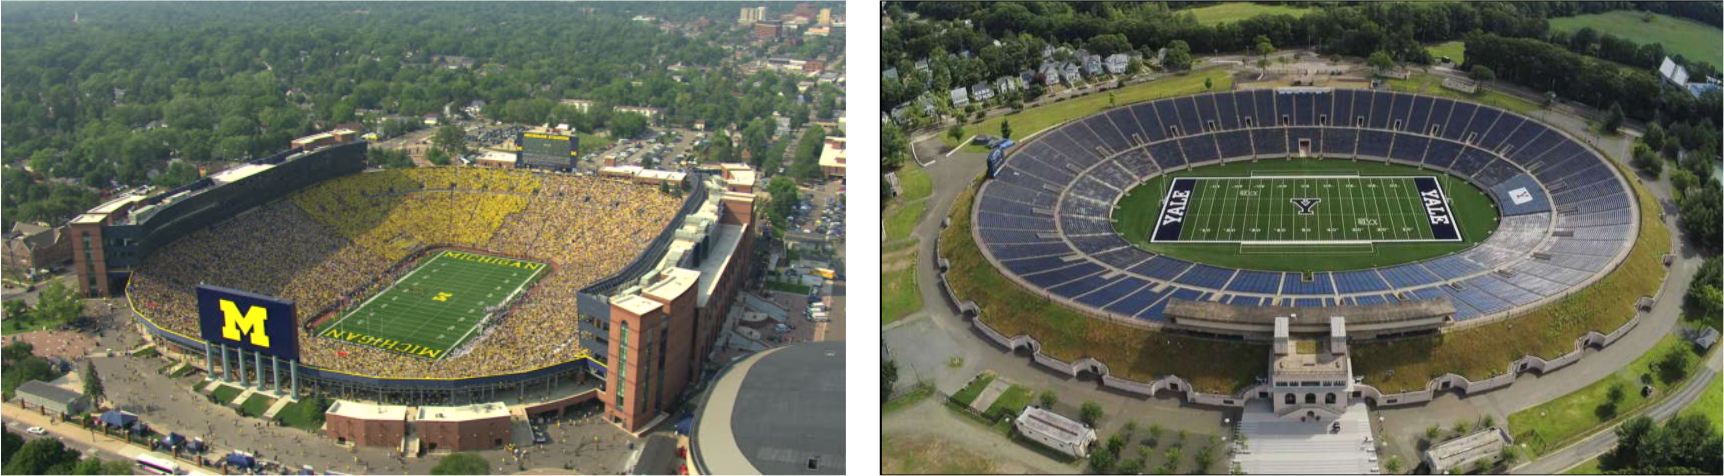
\includegraphics[width=23.94in]{figures/bighousebowl} \caption{Michigan Stadium (L), and the Yale Bowl}\label{fig:bighousebowl}
     \end{figure}
  \item
    Keep in mind, an HVAC systems take in air, condition it, then return it to the occupied space. It takes energy to motivate air to move. Moreover, people generally do not like feeling moving air when they are indoors.
  \end{enumerate}
\end{enumerate}

\hypertarget{calculations}{%
\section{Calculations}\label{calculations}}

\begin{enumerate}
\def\labelenumi{\arabic{enumi}.}
\tightlist
\item
  Develop worst-case scenarios for heating and cooling your stadium, eg, August and February days and nights, and calculate required rates of energy transfer. Outdoor conditions can be found in an almanac or NOAA climactic data.
\item
  Calculate the power required for an air conditioner or heat pump to meet cooling demands. Determine the cost of said power.
\item
  Calculate power requirements for a heat pump to satisfy heating demands. Compare heat pump power and cost to those of heating by natural gas and heating by pure electric Joule heating.
\item
  Calculate the time it takes your HVAC system to reach comfortable conditions, assuming the indoor environment is the same as outdoor ambient conditions.
\end{enumerate}

\hypertarget{report}{%
\section{Report}\label{report}}

\emph{coming soon}

\hypertarget{resources}{%
\section{Resources}\label{resources}}

\emph{coming soon}

\hypertarget{quick-chill}{%
\chapter{Quick Chill}\label{quick-chill}}

\textbf{N05-164, US Navy Request for Proposals}

\emph{Technology areas}\\
Materials/Processes, Human Systems

\emph{Objective}\\
Develop an energy efficient, rugged, shipboard capability to quickly chill a canned beverage product (e.g., soda pop, or ``soft drink'') to help eliminate the requirement for operating traditional vending machines at sea.

\hypertarget{project-summary}{%
\section{Project Summary}\label{project-summary}}

For the primary customer on a ship (male, 22 years old), a key Quality of Life (QOL) element as documented by customer surveys is the ability to obtain a cold soft drink from a vending machine. That the per capita consumption of the commodity is almost double the U.S. per capita rate (52 gal a year) testifies to the popularity and desirability of this service. To satisfy this demand, the Navy as part of its QOL programs provides soft drink vending machines on ships. The design of the ship (storerooms separated from selling locations) coupled with the lack of transportation aids and the requirement to have up to 14 machines on larger ships has driven large platforms to devote up to six (6) man-years of effort to keep the machines filled. As the cost of manpower has increased, the need to find alternatives to provide this key QOL product has grown.

The desire is to develop a device capable of chilling a soft drink within 10 seconds, which is estimated to be the upper limit, or customer wait time tolerance, for the beverage consumer. The militarized version of the device needs to be compact and reliable, with little or no in-service maintenance requirements. Such a device, when distributed throughout the shipboard environment, could provide the following benefits:

\begin{enumerate}
\def\labelenumi{\arabic{enumi}.}
\tightlist
\item
  Eliminate, or minimize, shipboard requirements for environmentally threatening use of refrigerants (o-zone deleting substances)\\
\item
  Potentially remove all labor requirements involved in the operation of vending machines.\\
\item
  Removing the requirement for the product to be chilled at the point-of-sale, enabling more purchasing and storage flexibility to both the retailer (Ship's Store) and the consumer (sailor)
\end{enumerate}

\hypertarget{background}{%
\section{Background}\label{background}}

The rapid chilling of bulk food products (e.g., dairy, fruits \& vegetables) and especially solid food (e.g., carcass meat, fresh fish) is a long sought-after industry endeavor that has posted modest advances, with futuristic sights on a capability akin to a ``reverse microwave''. Restricted by the same heat transfer principles, the objective to rapidly chill a packaged consumer beverage can proceed towards a similar outcome when, and if, technology pushes past the decades-old capability of the vending machine. Rapid chill, with chill-on-demand service, is an evolutionary step away from the trappings of 20th century vending technology.

Consumer appeal for a chill on demand capability is demonstrated in sales of counter-top, household products promising to chill a bottle of wine in six minutes, or a canned beverage in one minute. However, products currently known to be available are extremely limited in applicability, essentially relegated to home use given the need to add both water and ice to the device. Other chill-on-demand technologies include a self-refrigerating beverage can promising to cool 30 °F in three minutes.

While these two examples of technological applications demonstrate the variability in potential approaches for obtaining the desired objective, neither is close to the required shipboard solution (ease-of-use, adequate chilling within 10 seconds). In addition, before any organization will embrace a modern technology, it will determine if the cost of new technology is ``affordable'' either in acquisition cost or ``tradeoff'' cost of providing the current service. The shipboard technical requirement exceeds any technology known to be available in the marketplace, and therefore presents unusually high technical risk. For these reasons, some leeway may be accommodated for the desired objective considering the proposed study approaches received.

\hypertarget{project}{%
\section{Project}\label{project}}

Investigate alternative technologies/approaches to rapidly chill aluminum can packaged soft drinks/beverages. Evaluate and document alternatives and a developmental approach for one or more candidate devices.

A promising method is to have a chamber (or chambers) submerged in the drink. In the chamber is a fluid under pressure that will vaporize at atmospheric pressure and normal room temperature. When the chambers are opened, the fluid vaporizes. The Second Law demands the vaporization. The First Law demands the energy required for the phase change to take place. That energy is taken from anything in contact; it cannot be avoided. In this case, the energy is stolen from the soft drink, cooling it. \emph{Yes, this is what causes an aerosol can to get cold when sprayed.}

Other methods abound, but I'm less familiar with how they work. You're free to propose anything feasible. I'm willing to help you sort out your ideas as well.

\begin{enumerate}
\def\labelenumi{\arabic{enumi}.}
\tightlist
\item
  Develop a device capable of chilling a soft drink within 10 seconds.
\item
  Assume the soft drink is 12 fl.~oz. of water.\\
\item
  Assume the soft drink is initially 30,°C and must be chilled to 1,°C.
\item
  Use any of the substances tabulated in any textbook, ASHRAE manuals, NIST, etc.
\item
  Check for toxicity. I'm no advertising expert, but killing customers seems like it may potentially harm sales.
\end{enumerate}

\hypertarget{rocket-cryogenic-storage}{%
\chapter{Rocket Cryogenic Storage}\label{rocket-cryogenic-storage}}

\emph{under construction}

Storing Cryogenic liquids is a challenging endeavor.
Cryogenic liquids have boiling points that are far below ambient temperature.
When storing them, a major challenge is reducing boil-off.
The cryogen is under saturation conditions.
Any heat transfer into the tank causes some of the cryogen to boil away, a serious concern for applications that requires liquid cryogen (as opposed to very cold gas).

Consider a rocket fueled by liquid methane (LMG), with liquid oxygen (LOX) oxidizer.
You are charged with designing the fuel system.
We've already determined how much fuel and oxidizer are required to complete the mission. Your major concern is the loss of LMG and LOX while the rocket sits on the pad. You will be launching from the New Mexico desert in mid-June, and the rocket may sit on the pad for up to 2 hours after fueling.
Because you're so good at thermodynamics, you know you have several options at your disposal:

\begin{enumerate}
\def\labelenumi{\arabic{enumi}.}
\tightlist
\item
  Increase tank pressure.
\item
  Insulate the tanks.
\item
  Load extra cryogens.
\end{enumerate}

\hypertarget{this-isnt-rocket-science}{%
\section{This isn't rocket science\ldots{}}\label{this-isnt-rocket-science}}

\hypertarget{its-rocket-engineering}{%
\section{\ldots it's rocket engineering}\label{its-rocket-engineering}}

\begin{figure}

{\centering 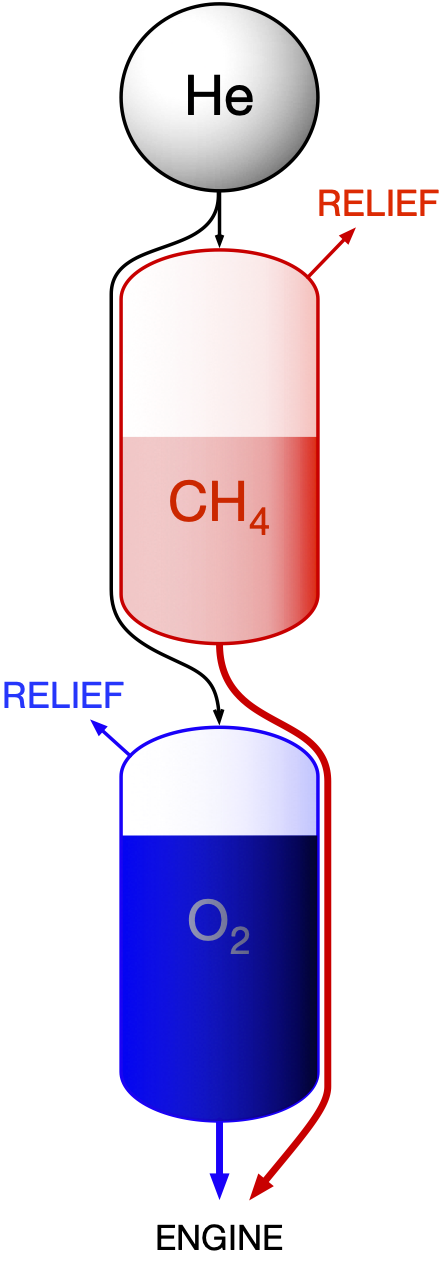
\includegraphics[width=0.25\linewidth]{./figures/rocket-fuel} 

}

\caption{Simple depiction of a rocket fuel system}\label{fig:rocket-fuel}
\end{figure}

\hypertarget{project}{%
\section{Project}\label{project}}

\begin{enumerate}
\def\labelenumi{\arabic{enumi}.}
\tightlist
\item
  Size both tanks.
\item
  Specify the initial masses of LOX and LMG to be loaded into each tank. This is the amount before any boiloff begins.
\item
  Specify operating pressure of each tank.
\item
  Specify the insulation and its thickness.
\end{enumerate}

\hypertarget{constraints-and-requirements}{%
\section{Constraints and requirements}\label{constraints-and-requirements}}

\begin{enumerate}
\def\labelenumi{\arabic{enumi}.}
\tightlist
\item
  It's a rocket. Low weight is holy and just.
\end{enumerate}

\hypertarget{resources}{%
\section{Resources}\label{resources}}

You may need property data beyond what is in your textbook. Feel free to use other texts, ASHRAE Handbooks, etc. Mathematica has a very nice thermodynamic properties function. The NIST \citep{linstrom_nist_2019} Chemistry WebBook may be a good option. Find it at \url{webbook.nist.gov}.

\hypertarget{heat-transfer}{%
\section{Heat Transfer}\label{heat-transfer}}

\hypertarget{home-energy-audit}{%
\chapter{Home Energy Audit}\label{home-energy-audit}}

\emph{under coonstruction}

\hypertarget{stirling-engine}{%
\chapter{Stirling Engine}\label{stirling-engine}}

Build a working Stirling engine powered by a candle.

\hypertarget{waste-to-energy}{%
\chapter{Waste-to-Energy}\label{waste-to-energy}}

\emph{under construction}

Kill a flock of birds with one rock and a good throw.

\hypertarget{waste-heat-recovery}{%
\chapter{Waste Heat Recovery}\label{waste-heat-recovery}}

\emph{under construction}

\hypertarget{writing-a-great-technical-report}{%
\chapter{\texorpdfstring{Writing a \textbf{\emph{Great}} Technical Report}{Writing a Great Technical Report}}\label{writing-a-great-technical-report}}

\emph{under construction}

\hypertarget{pain-peril-promise}{%
\section{Pain, peril, promise}\label{pain-peril-promise}}

\begin{enumerate}
\def\labelenumi{\arabic{enumi}.}
\tightlist
\item
  Abstract/Summary
\item
  Pain
\item
  Attempted solutions
\item
  Promise
\item
  Work
\item
  Results
\item
  Well\ldots?
\item
  Now what?
\end{enumerate}

  \bibliography{book.bib,packages.bib}

\end{document}
